\section*{CHƯƠNG 4: KẾT QUẢ THỰC HIỆN}
\addcontentsline{toc}{section}{\numberline {} CHƯƠNG 4: KẾT QUẢ THỰC HIỆN}
\setcounter{section}{4}
\setcounter{figure}{0}
\setcounter{subsection}{0}
\subsection{KẾT QUẢ THI CÔNG PHẦN CỨNG}
Mô hình phần cứng của đồ án này bao gồm, 2 node Arduino giao tiếp với gateway Raspberry thông qua mạng LoRa để truyền các dữ liệu cảm biến như nhiệt độ, độ ẩm, ... ở node ao tôm và node vườn thanh long. Đồng thời nhận lệnh điều khiển từ gateway để bật tắt 2 relay "Máy bơm nước" và "Đèn" ở node vườn thanh long. Dưới đây là ảnh minh hoạ cho mô hình truyền/nhận của phần cứng:
\begin{figure}[H]
	\centering
	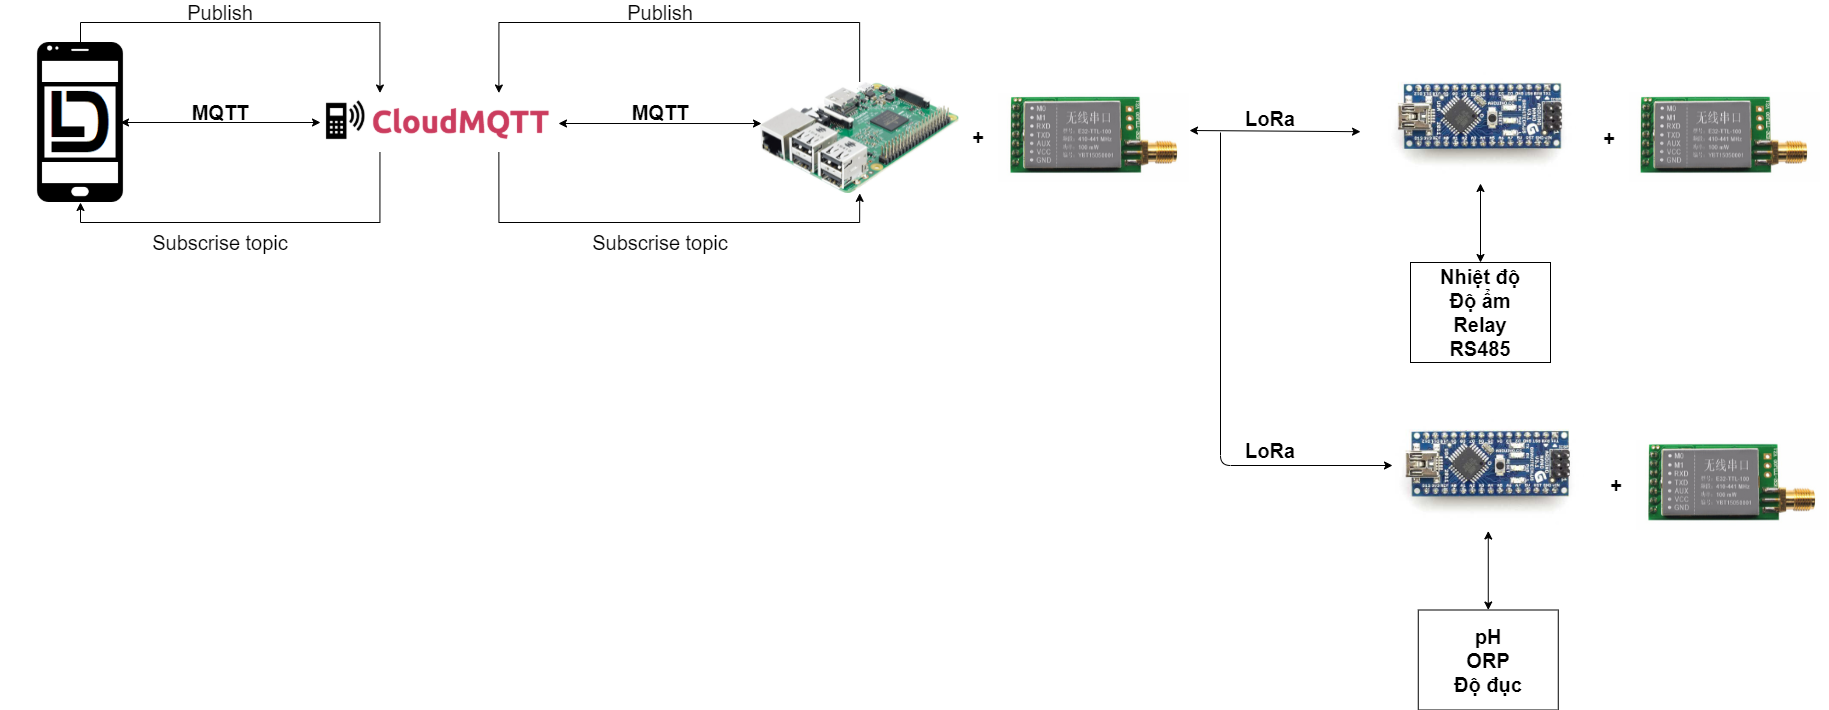
\includegraphics[scale=0.2]{Chapter 4/image chapter 4/sodoDCLV.png}
	\caption[Sơ đồ các giao tiếp phần cứng]{Sơ đồ các giao tiếp phần cứng}
	\label{hinh41}
\end{figure}
\subsubsection{Hình ảnh phần cứng thực tế của node đặt ở vườn thanh long}
\indent Do vẫn còn phát triển thêm: gắn thêm cảm biến, thay thế 1 số linh kiện cho phù hợp, ... Nên em vẫn còn dùng bread board để cắm mạch cho tiện việc nghiên cứu. Trong tương lai, khi tiến hành phát triển lên Luận văn Tốt nghiệp, em sẽ đưa mạch này lên PCB.
\begin{figure}[H]
	\centering
	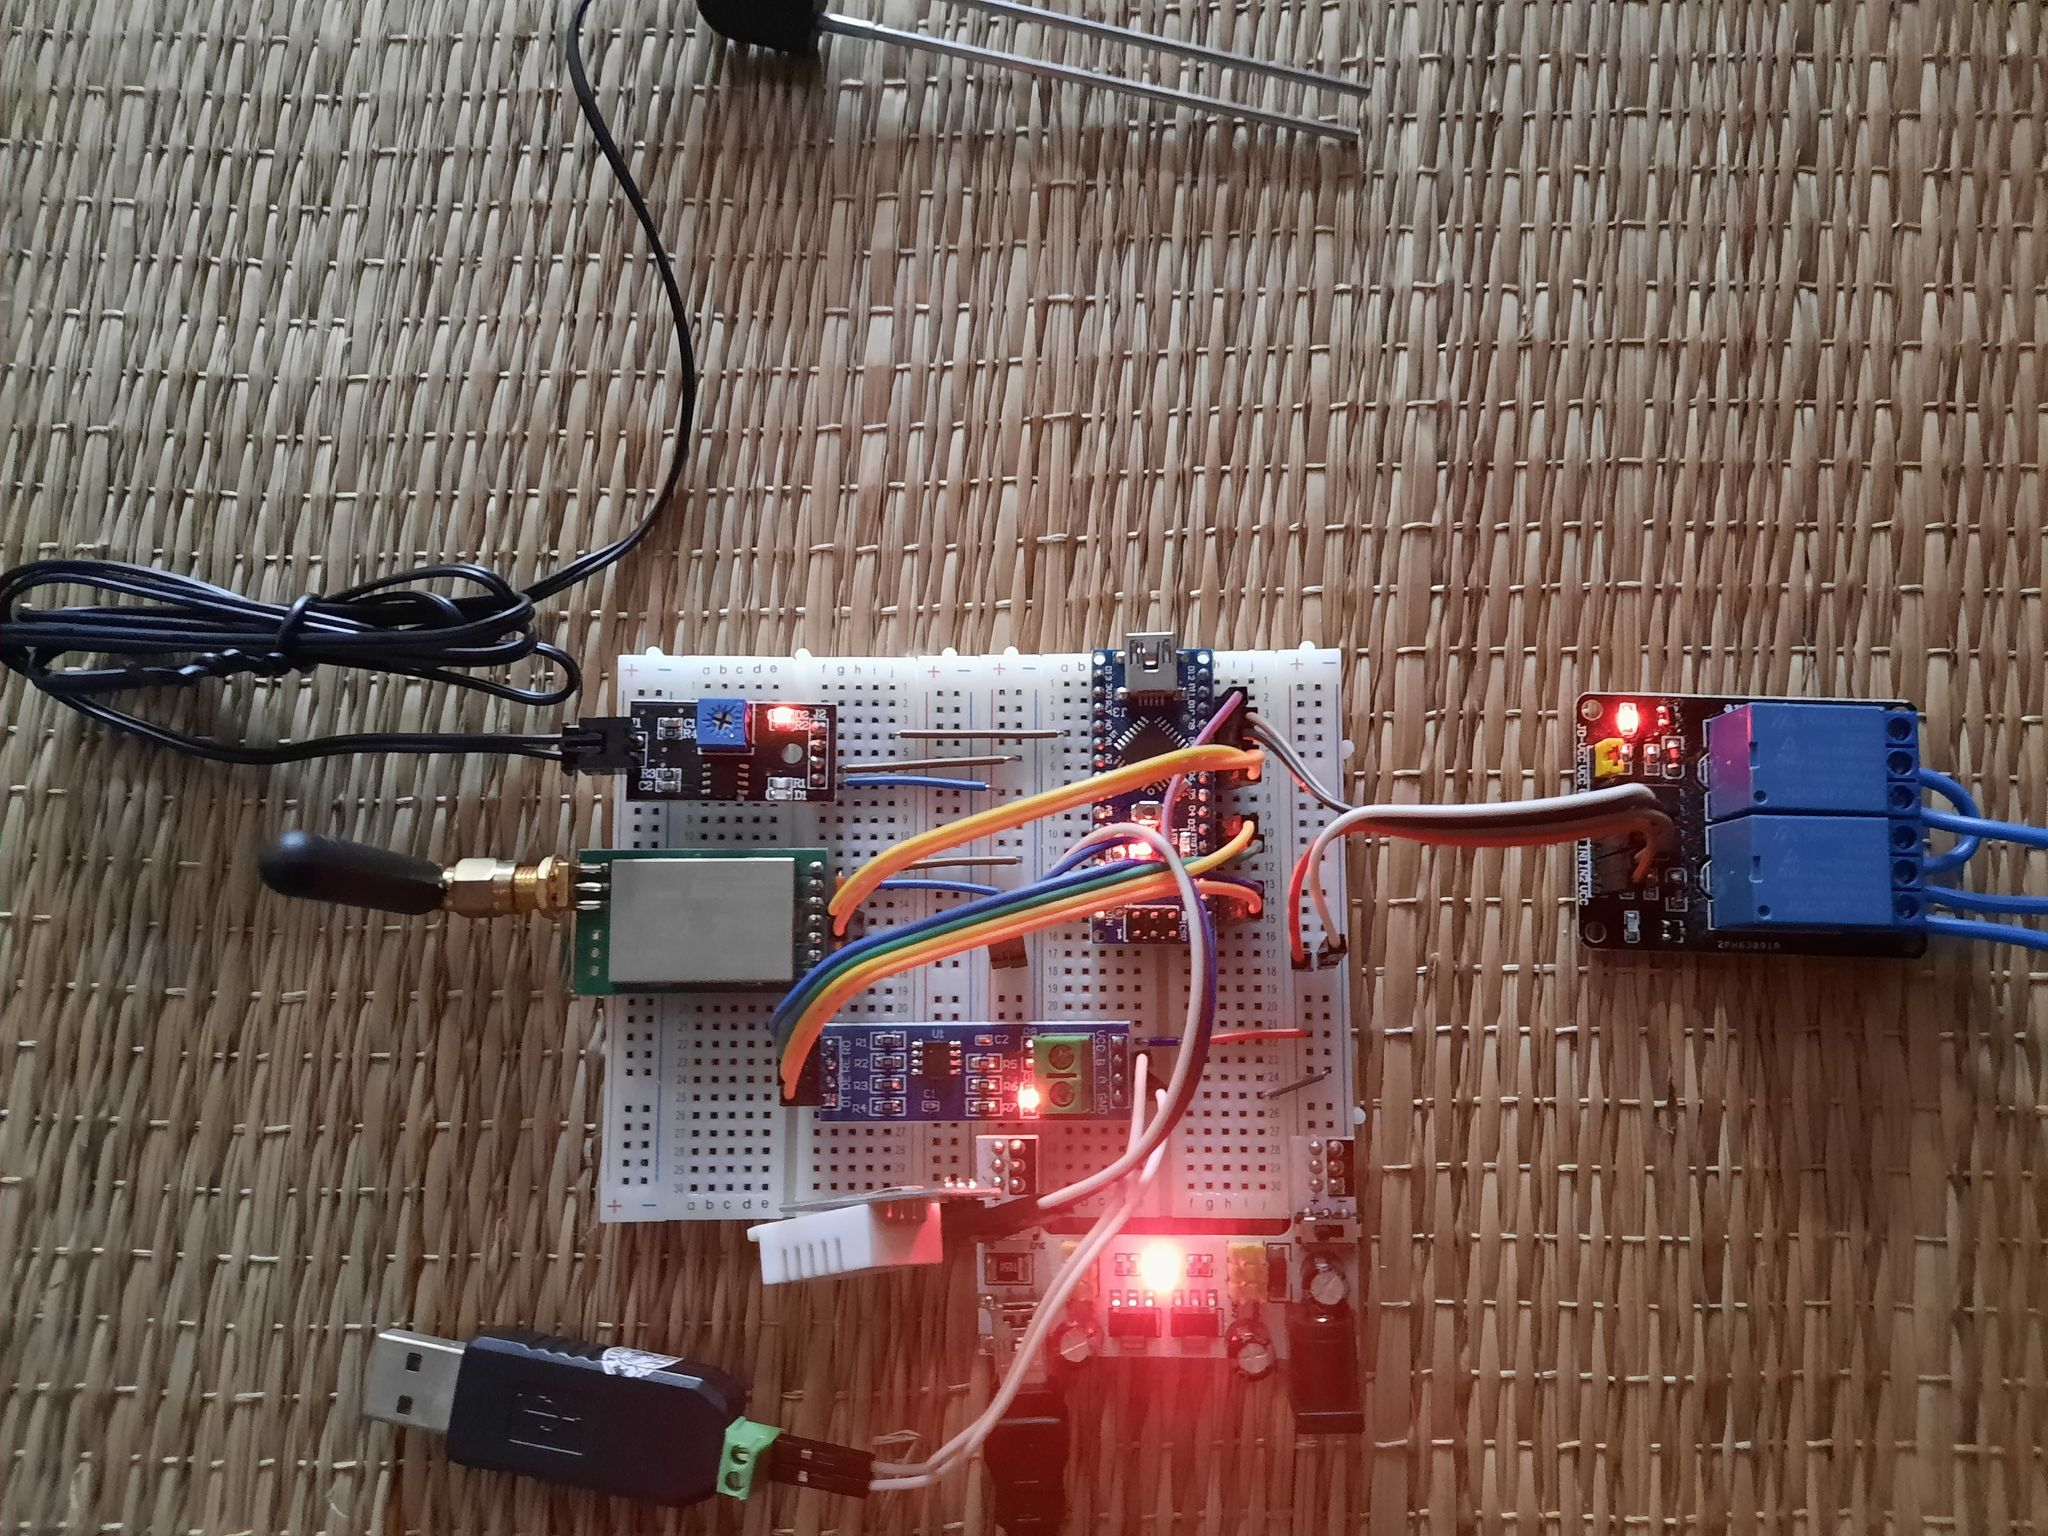
\includegraphics[scale=0.1]{Chapter 4/image chapter 4/phancung.jpg}
	\caption[Phần cứng node vườn thanh long thực tế]{Phần cứng node vườn thanh long thực tế}
	\label{hinh42}
\end{figure}
\subsubsection{Hình ảnh phần cứng thực tế của node đặt ở ao tôm}
\indent Node đặt ở ao tôm, được em đầu tư đóng hộp để bảo vệ các linh kiện điện tử bên trong, cũng như hạn chế được các tác động của môi trường, thời tiết bên ngoài tác động, ảnh hưởng đến độ bền và khả năng hoạt động của hệ thống bên trong.
\begin{figure}[H]
	\centering
	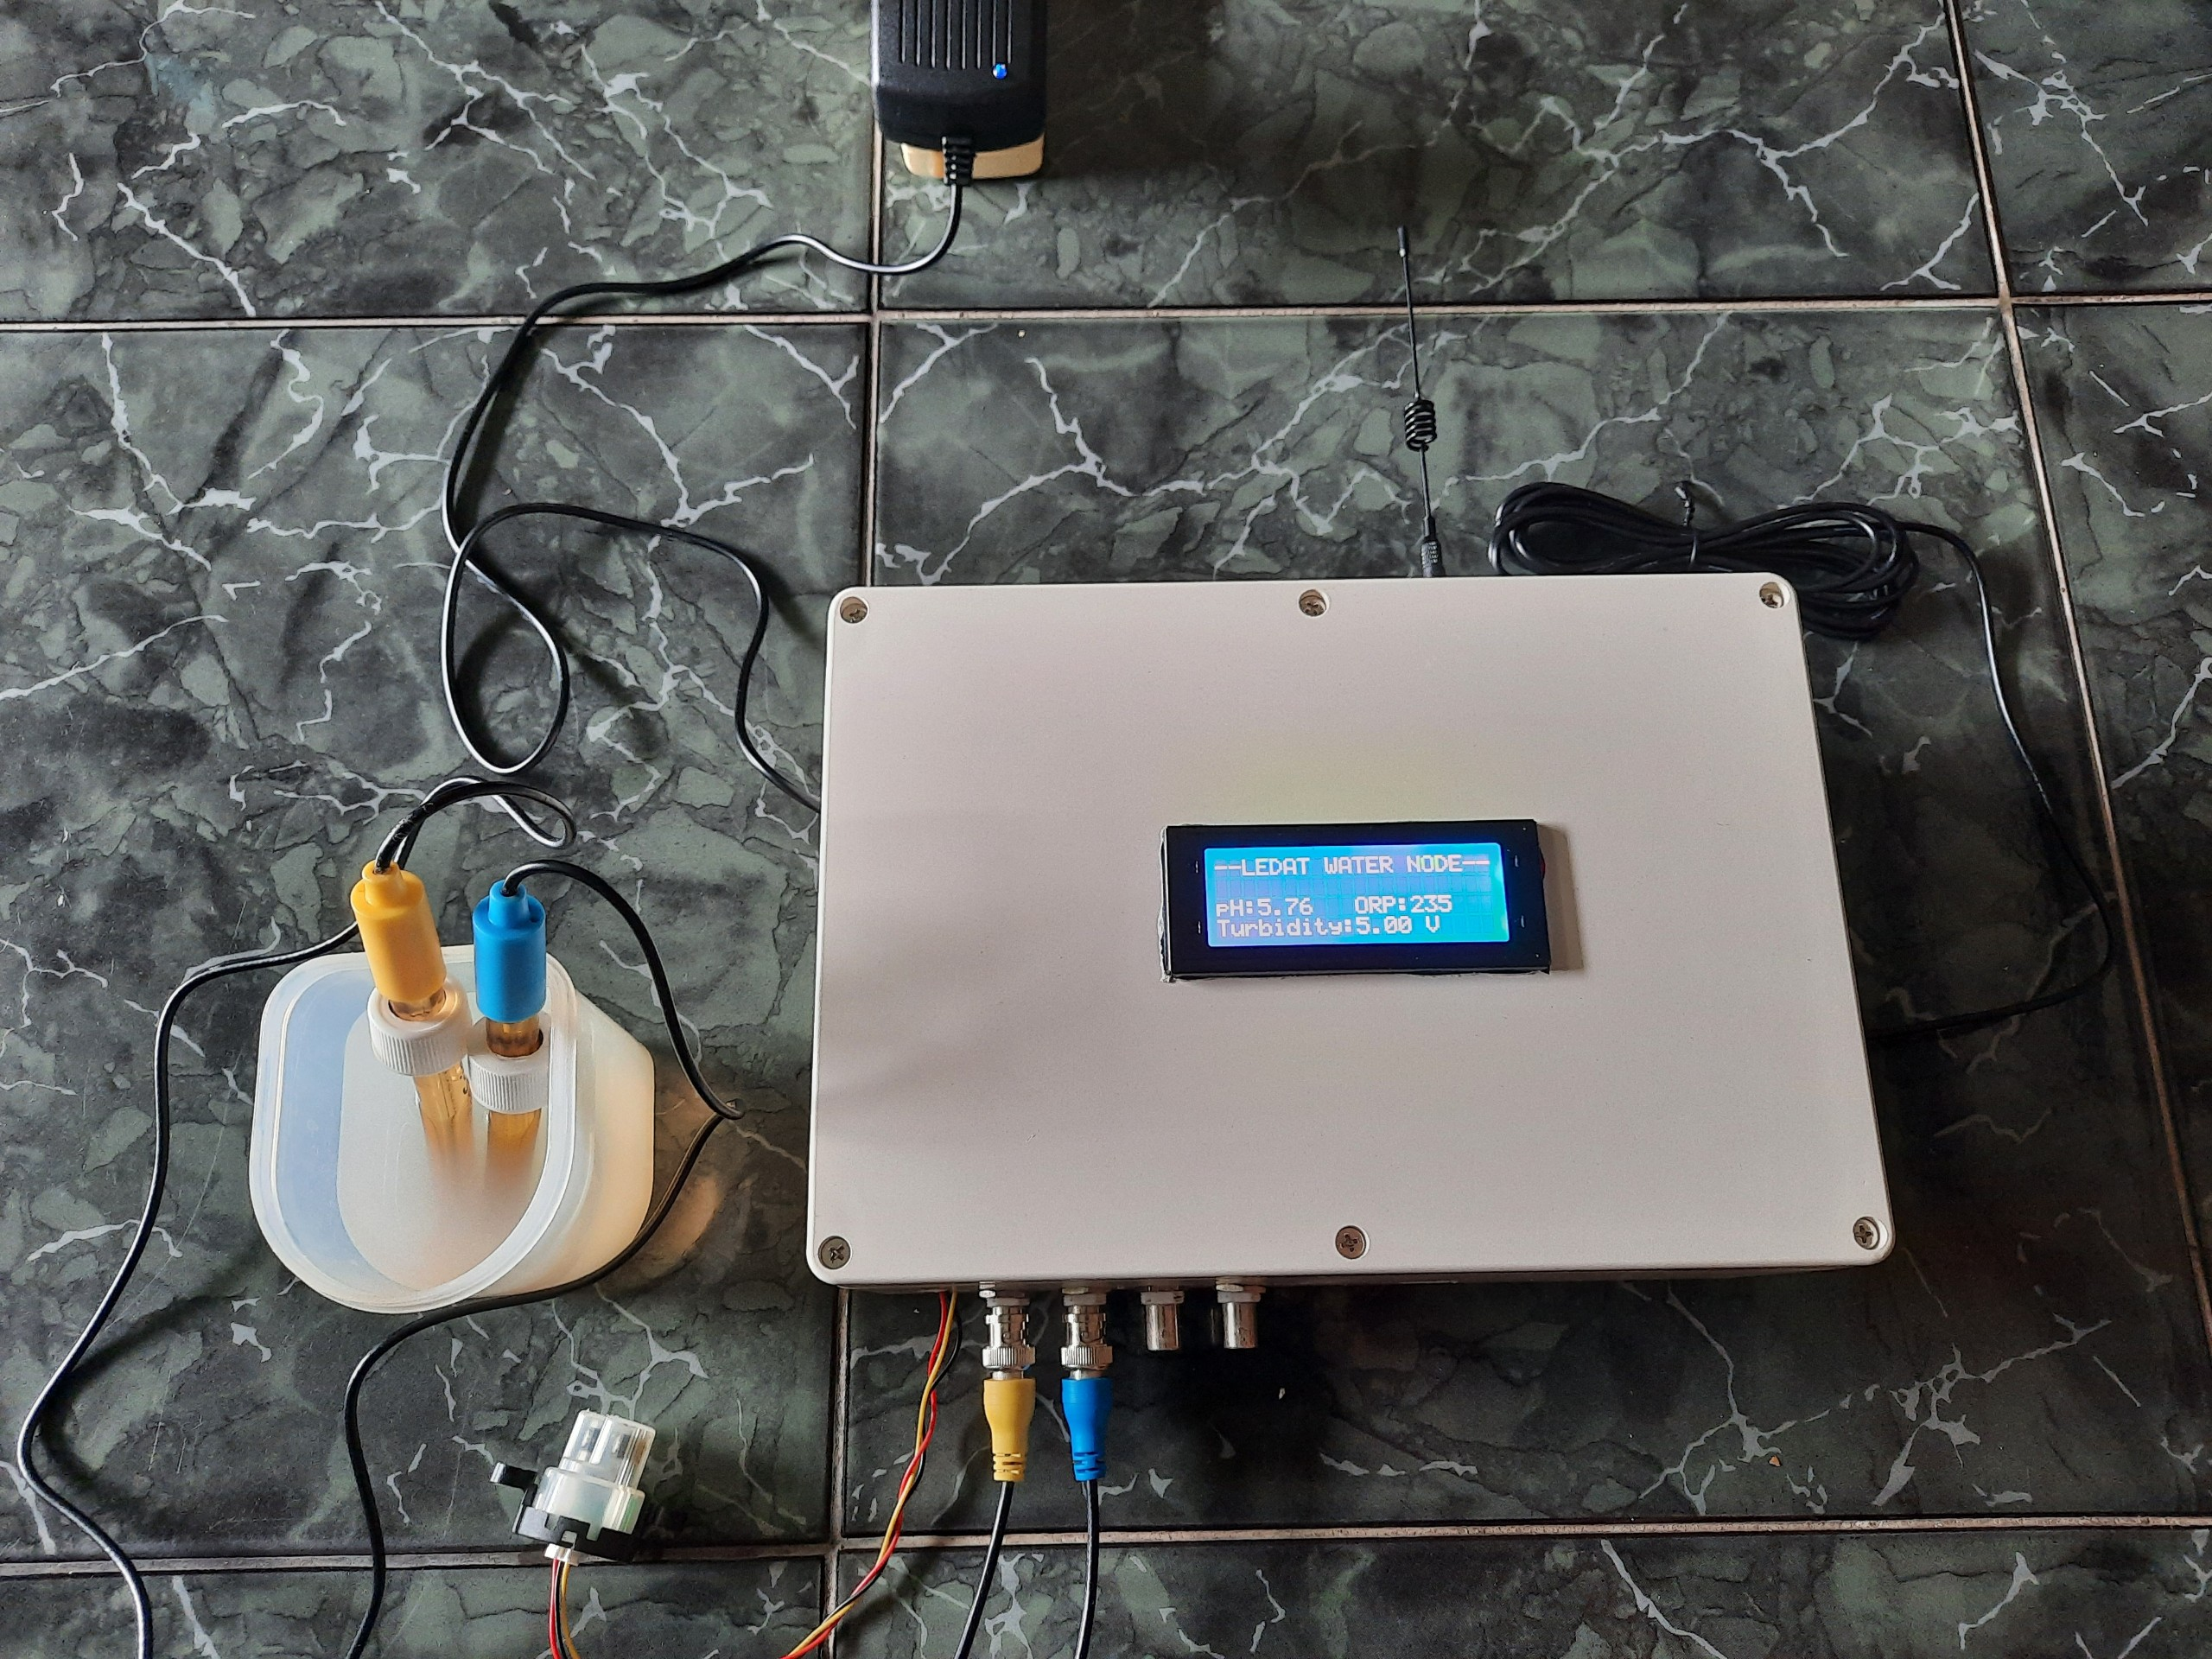
\includegraphics[scale=0.1]{Chapter 4/image chapter 4/aotomNode.jpg}
	\caption[Phần cứng node ao tôm thực tế]{Phần cứng node ao tôm thực tế}
\end{figure}
\indent Anten được bố trí phía trên hộp để đảm bảo node có thể truyền nhận dữ liệu 1 cách tốt nhất, Anten đã được nâng cấp lên Anten GSM 9dbi SMA Đực để tăng khả năng giao tiếp. Trong tương lai, em cũng sẽ nâng cấp anten của node vườn thanh long tương tự như vậy.
\begin{figure}[H]
	\centering
	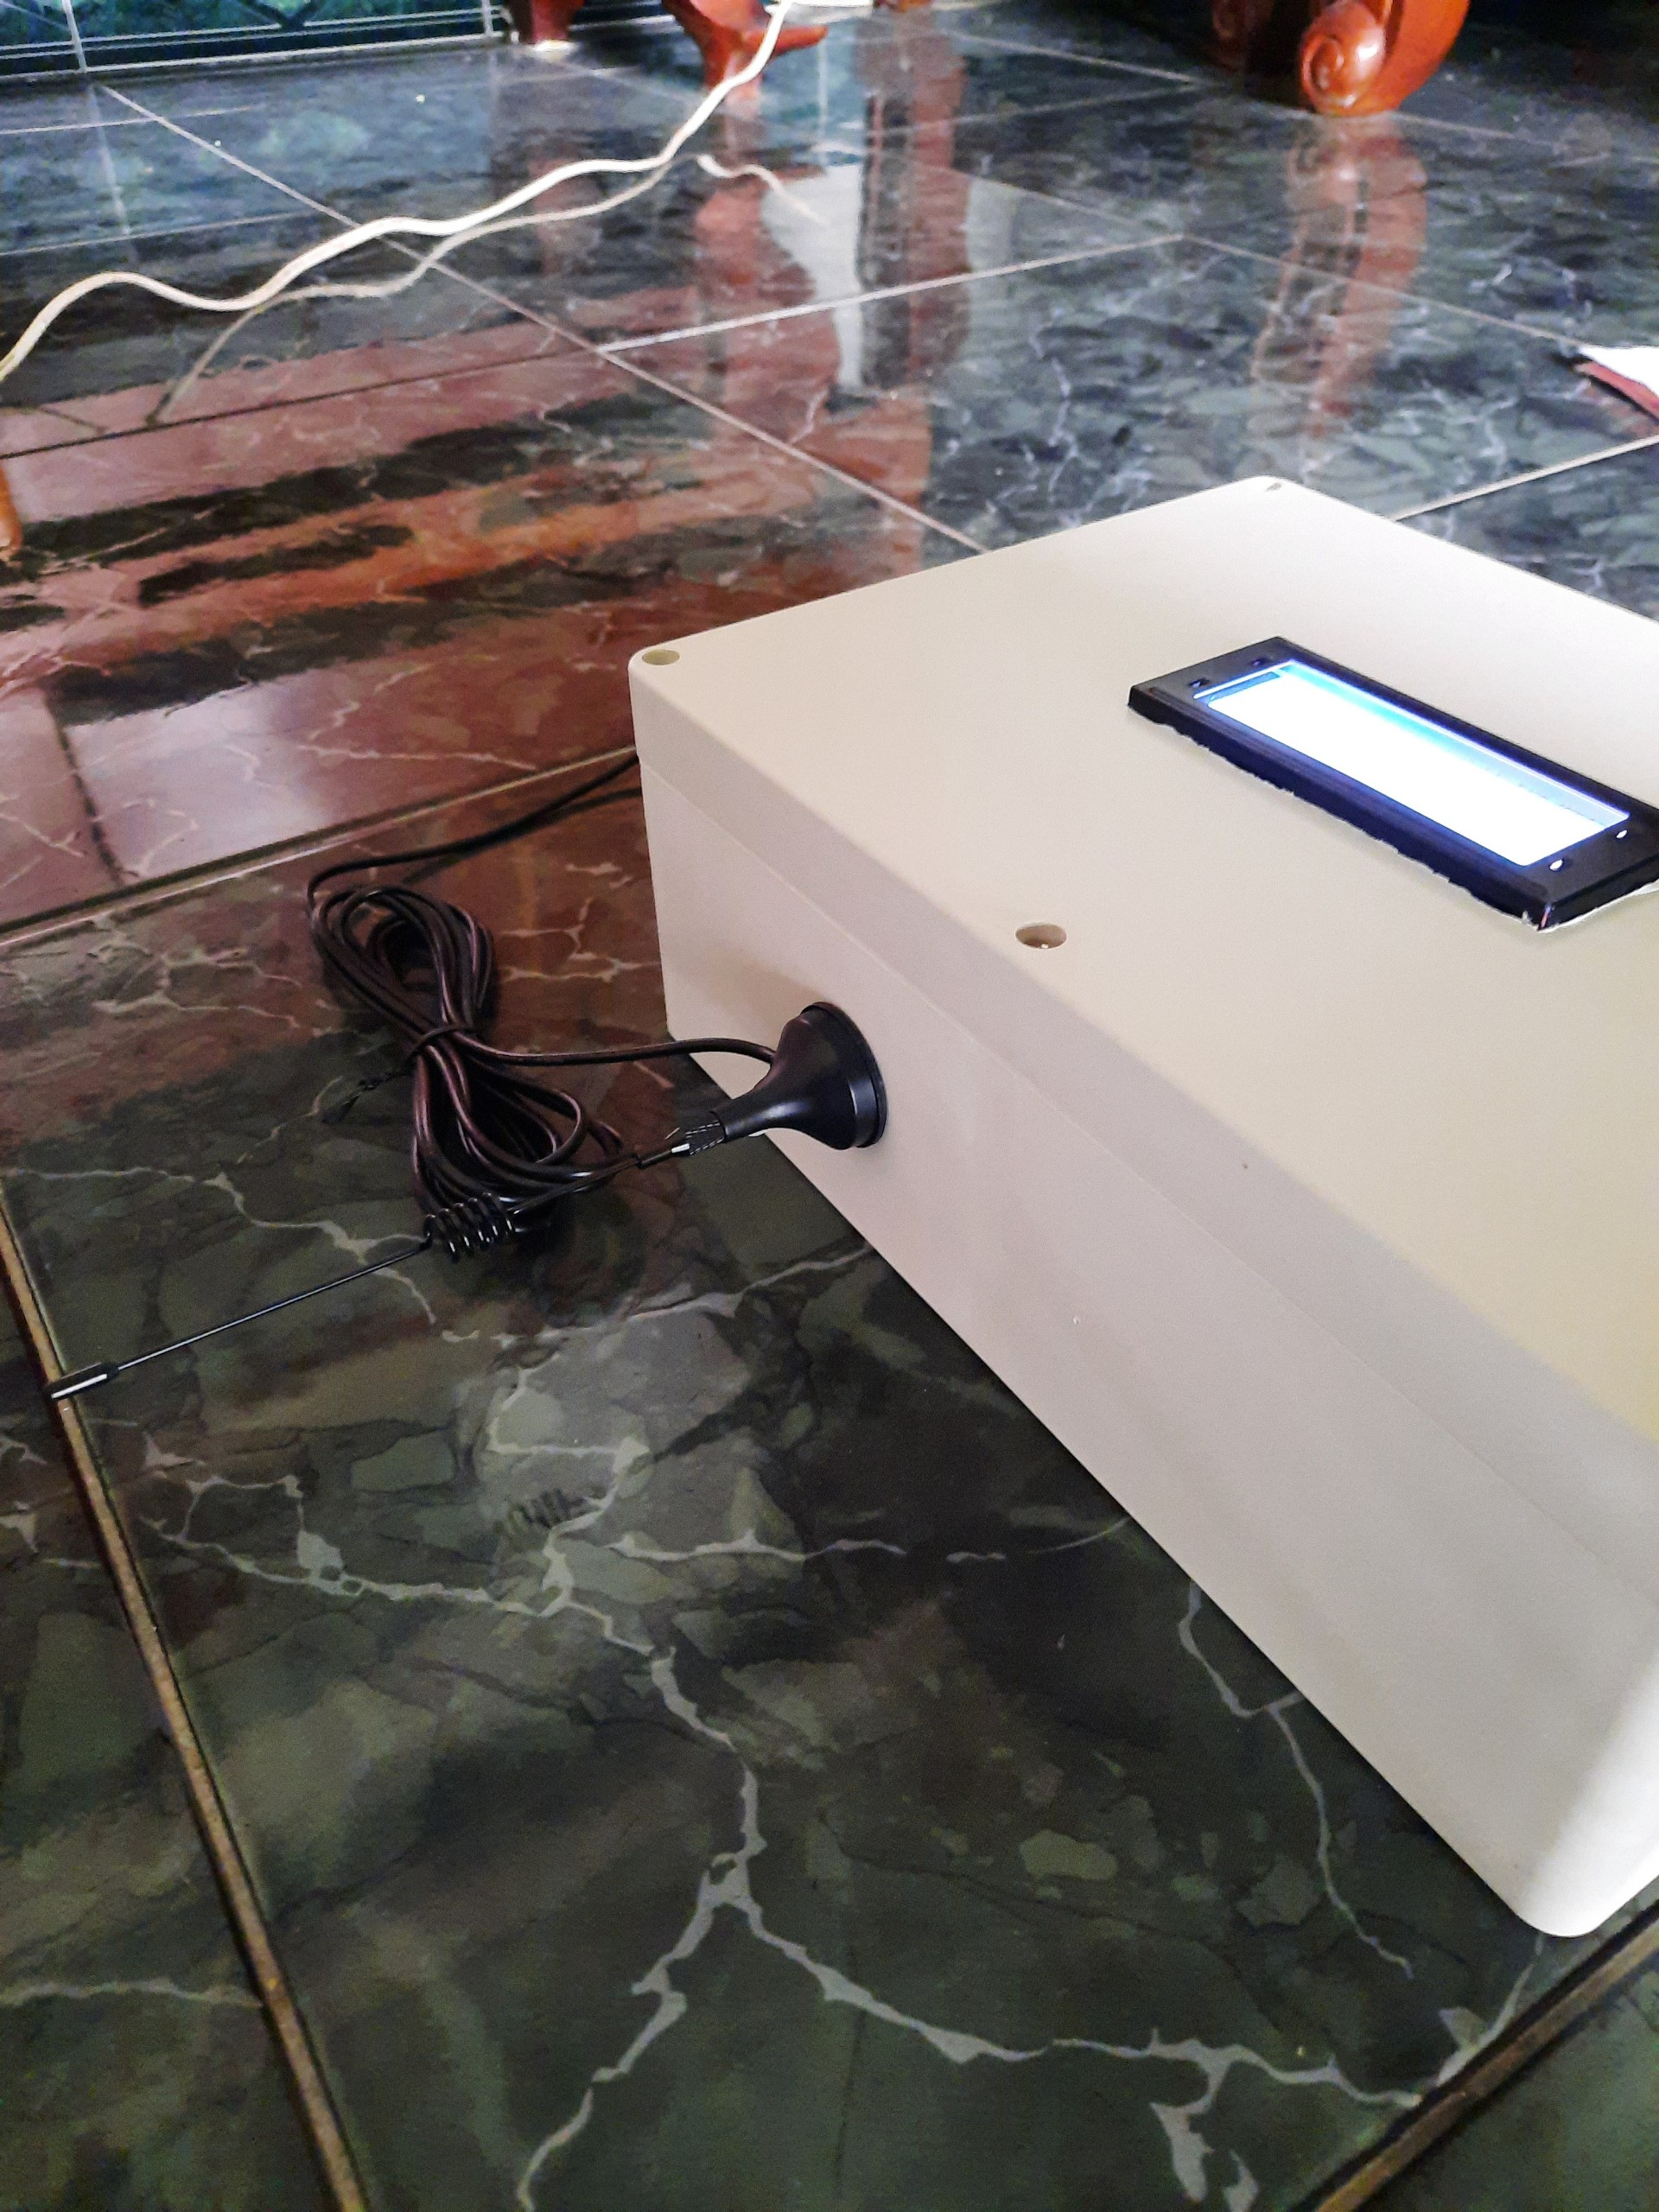
\includegraphics[scale=0.1]{Chapter 4/image chapter 4/antenAotom.jpg}
	\caption[Phần cứng node ao tôm thực tế]{Phần cứng node ao tôm thực tế}
\end{figure}
\subsection{KIỂM TRA CÁC THÔNG SỐ MÔI TRƯỜNG THU ĐƯỢC TỪ 2 NODE}
Dưới đây là hình ảnh được hiển thị trên App và Gateway cho ta biết các giá trị được 2 node Arduino thu về từ cảm biến và truyền lại cho gateway thông qua sóng LoRa.\\
\indent Với các thông số của môi trường thu về được từ 2 node như sau:
\begin{itemize}
	\item \textbf{\textit{Nhiệt độ: }} 31*C
	\item \textbf{\textit{Độ ẩm không khí: }} 60\%
	\item \textbf{\textit{Độ ẩm đất: }} 0\% (do cảm biến độ ẩm đất chưa được cắm vào đất)
	\item \textbf{\textit{Độ pH của nước: }} 11 (môi trường thử nghiệm là môi trường nước javel)
	\item \textbf{\textit{Chỉ số oxi hoá khử: }} 486
	\item \textbf{\textit{Độ đục của nước: }} 0V (do cảm biến đang được đặt trên môi trường không khí chưa được cho vào môi trường nước đục)
\end{itemize}

\begin{figure}[H]
	\centering
	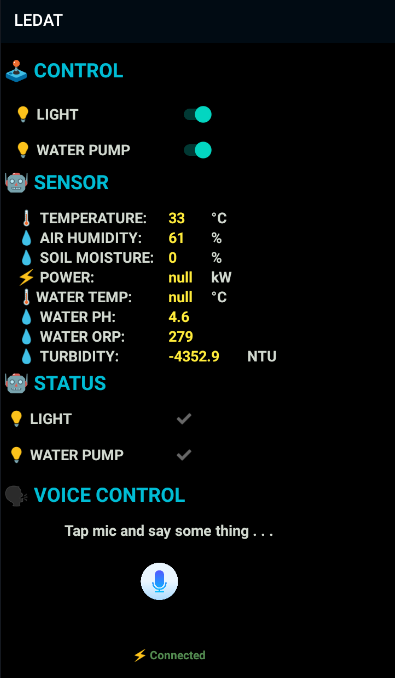
\includegraphics[scale=0.4]{Chapter 4/image chapter 4/appMT.png}
	\caption[Các thông số của môi trường được hiển thị trên app]{Các thông số của môi trường được hiển thị trên app}
	\label{hinh43}
\end{figure}
\begin{figure}[H]
	\centering
	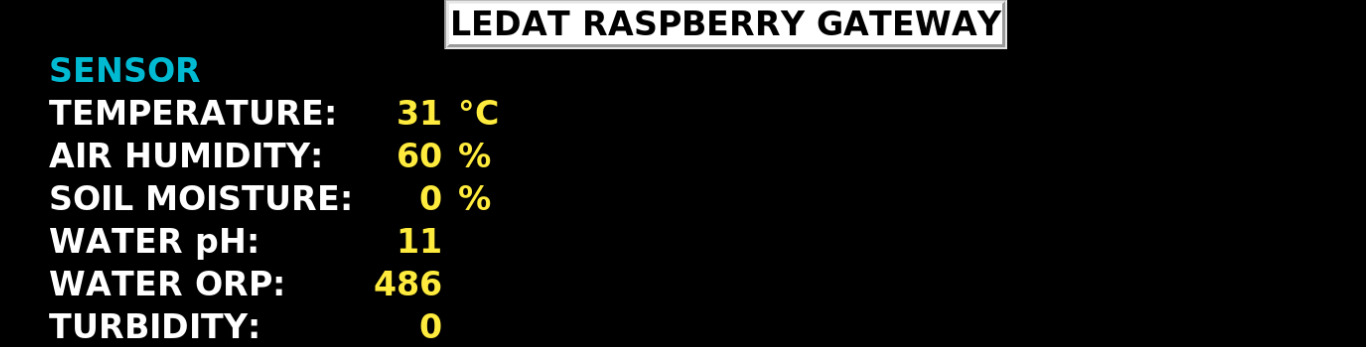
\includegraphics[scale=0.4]{Chapter 4/image chapter 4/gwMT.png}
	\caption[Các thông số của môi trường được hiển thị trên Gateway]{Các thông số của môi trường được hiển thị trên Gateway}
	\label{hinh44}
\end{figure}
\subsection{KIỂM TRA HOẠT ĐỘNG CỦA NODE AO TÔM}
\indent Các thông số từ cảm biến được hiển thiện trên màn hình LCD 20x4 tiện lợi cho việc theo dõi trực tiếp các thông số mà không cần thông qua quan sát trên Gateway.
\begin{figure}[H]
	\centering
	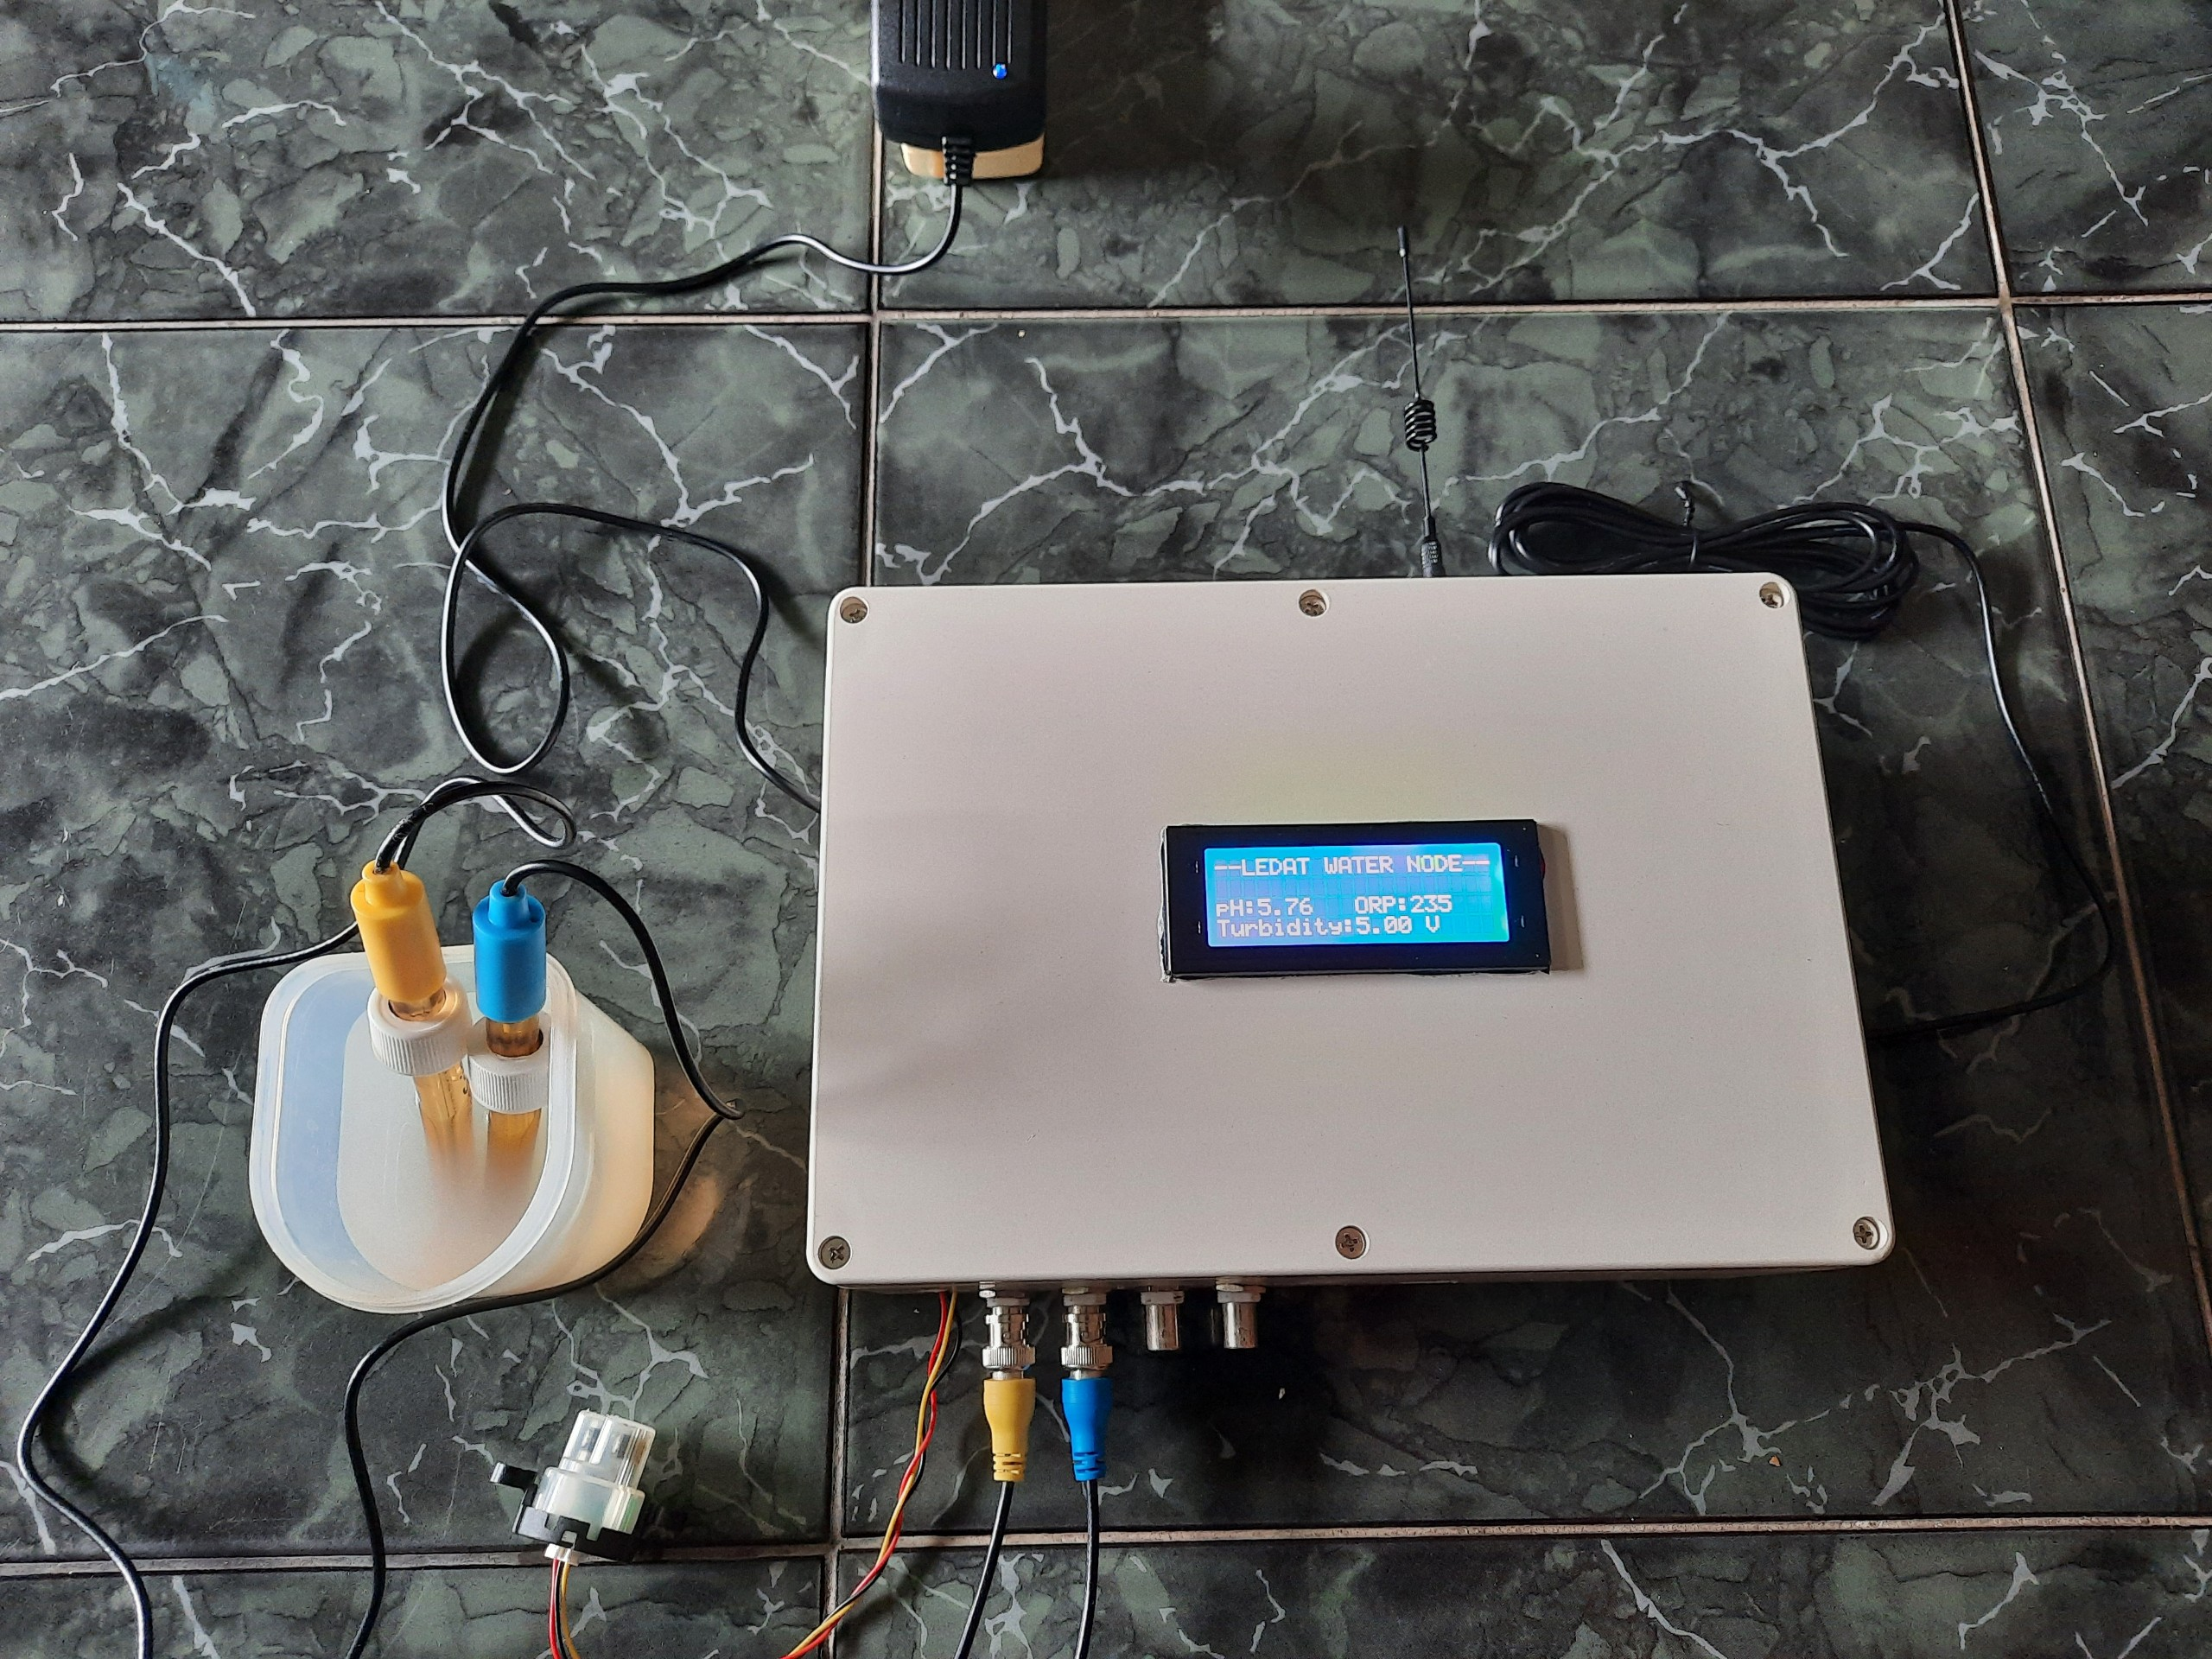
\includegraphics[scale=0.1]{Chapter 4/image chapter 4/aotomNode.jpg}
	\caption[Các thông số của môi trường nước được cảm biến thu về và hiển thị trên màn hình LCD]{Các thông số của môi trường nước được cảm biến thu về và hiển thị trên màn hình LCD}
\end{figure}
\subsection{KIỂM TRA HOẠT ĐỘNG CỦA MODULE 2 RELAY}
Ta tiến hành thử nghiệm bằng cách bật relay 1. Dưới đây là hình ảnh phần cứng phản hồi lại lệnh điều khiển bật relay 1 nhận từ Gateway truyền về thông qua LoRa.
\begin{figure}[H]
	\centering
	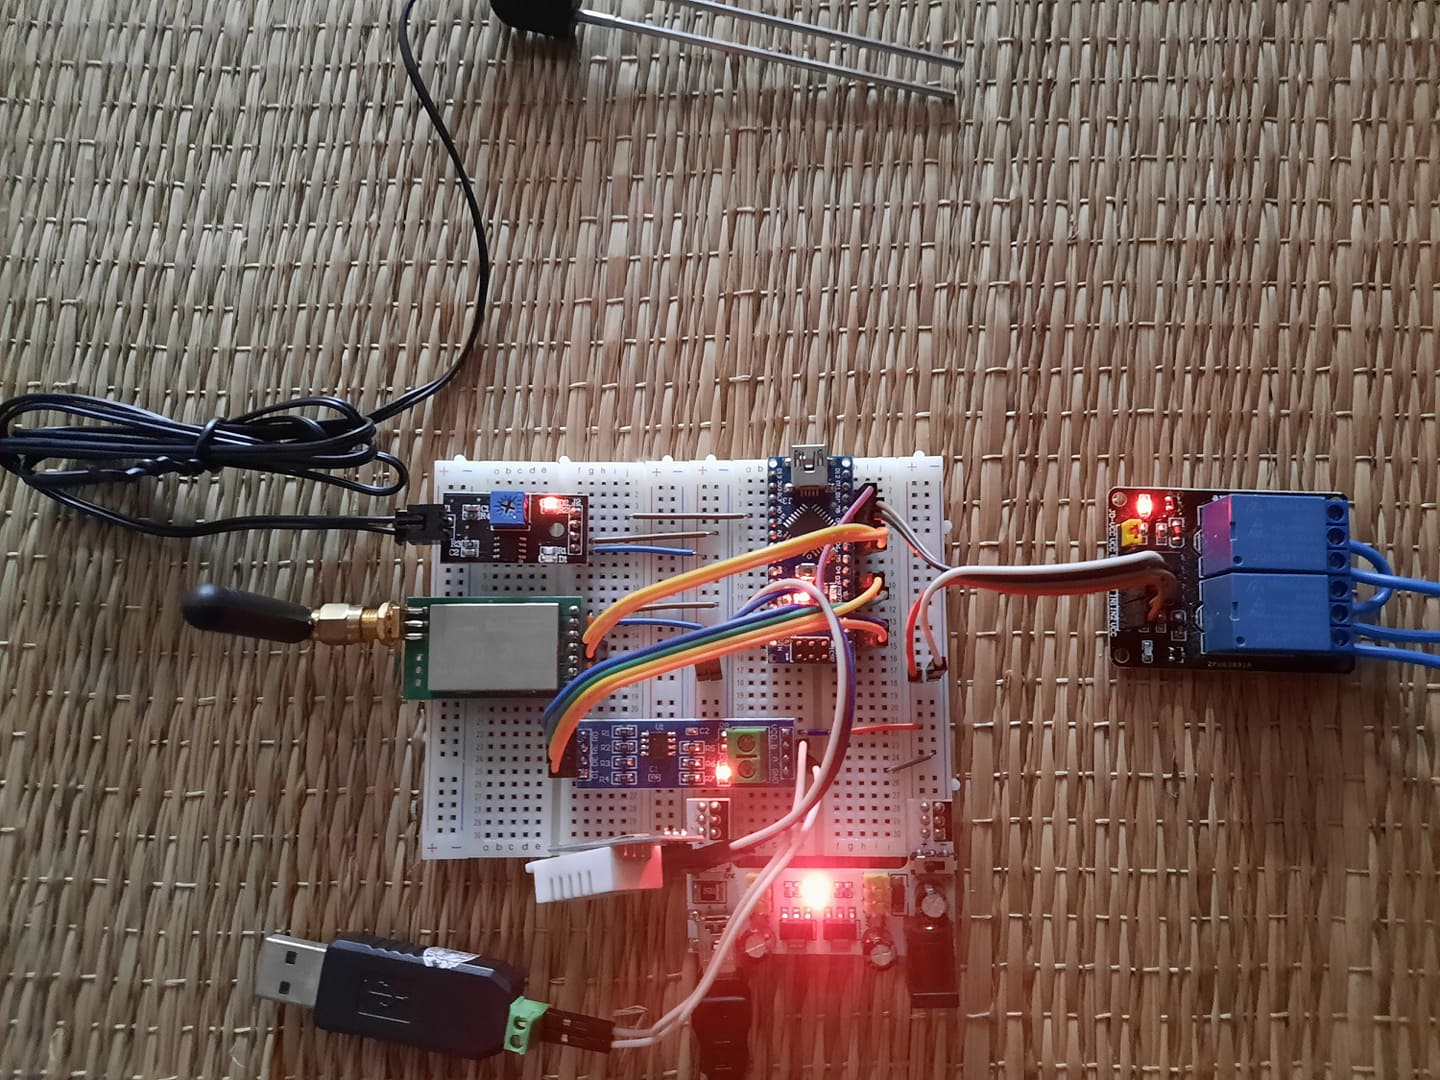
\includegraphics[scale=0.2]{Chapter 4/image chapter 4/R1ONR2OFF.jpg}
	\caption[Phần cứng trong trạng thái bật relay 1 tắt relay 2]{Phần cứng trong trạng thái bật relay 1 tắt relay 2}
	\label{hinh45}
\end{figure}
\indent Giao diện trên app đã hiển thị được các thông số của môi trường cũng như trạng thái bật/tắt của 2 thiết bị tại relay 1 và relay 2
\begin{figure}[H]
	\centering
	
\includegraphics[scale=0.2]{Chapter 4/image chapter 4/appR1ONR2OFF.png}
	\caption[Trang thái của end-Node được hiển thị trên app]{Trang thái của end-Node được hiển thị trên app}
	\label{hinh46}
\end{figure}
\indent Giao diện trên Gateway cũng đã hiển thị được các thông số của môi trường và trạng thái của 2 relay.
\begin{figure}[H]
	\centering
	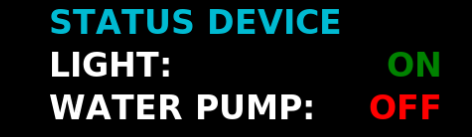
\includegraphics[scale=0.3]{Chapter 4/image chapter 4/Relay1ON-Relay2OFF.png}
	\caption[Trang thái của end-Node được hiển thị trên Gateway]{Trang thái của end-Node được hiển thị trên Gateway}
	\label{hinh47}
\end{figure}
\indent Tương tự, ta tiến hành thử nghiệm bật relay 2 và tắt relay 1.
\begin{figure}[H]
	\centering
	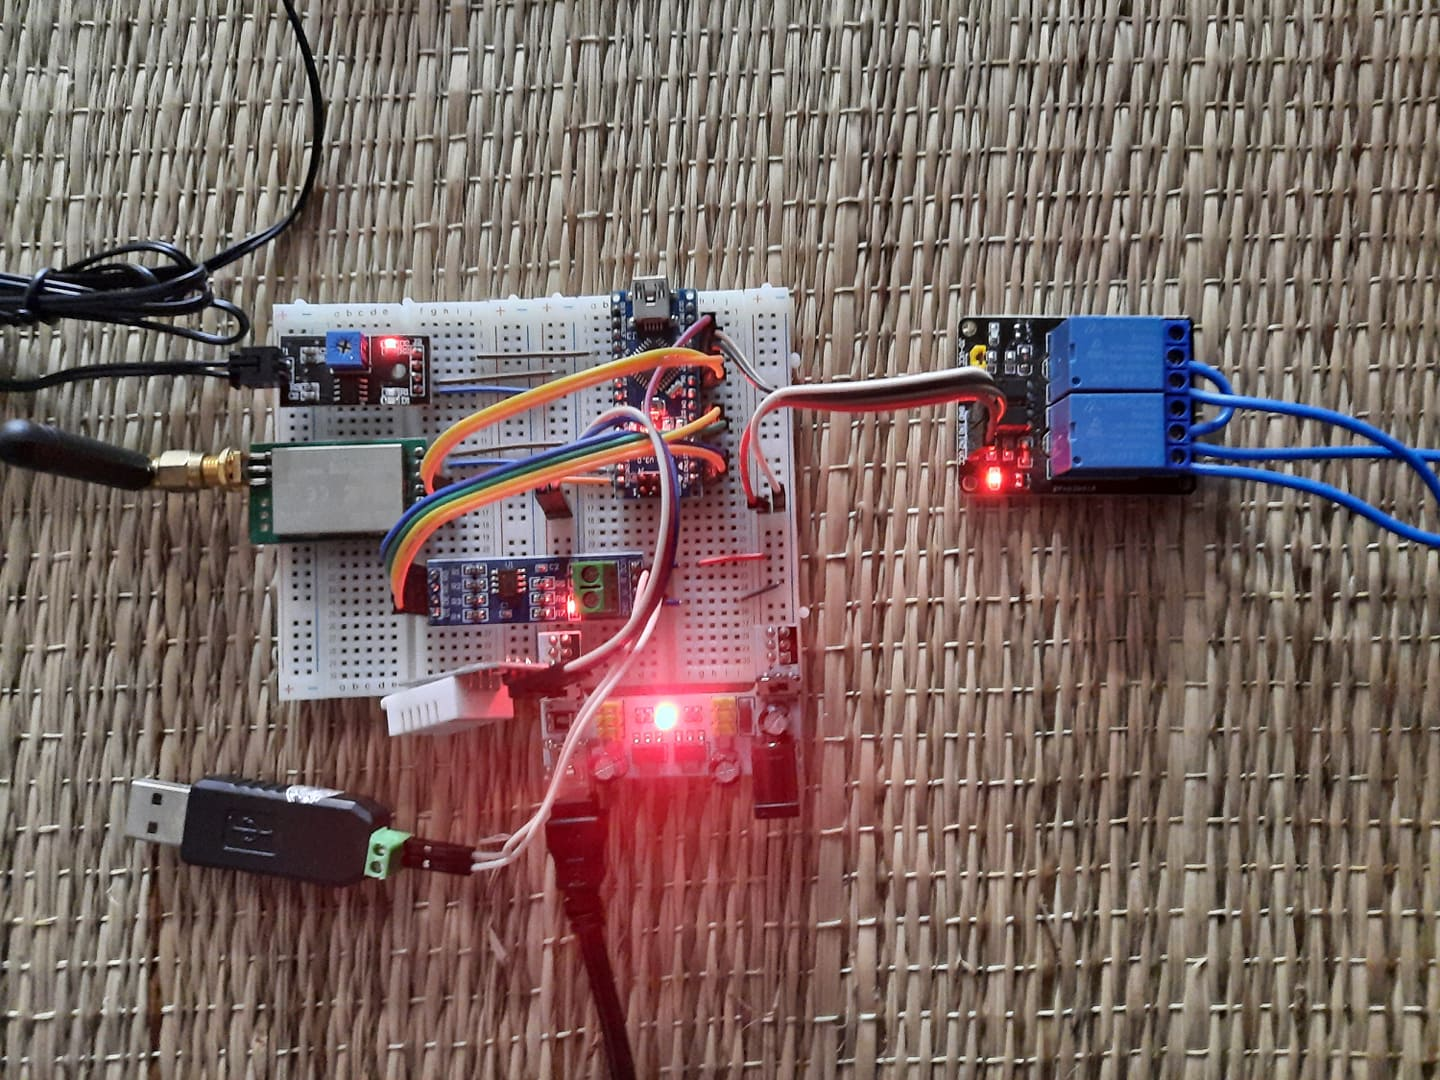
\includegraphics[scale=0.2]{Chapter 4/image chapter 4/R2ONR1OFF.jpg}
	\caption[Phần cứng trong trạng thái bật relay 2 tắt relay 1]{Phần cứng trong trạng thái bật relay 2 tắt relay 1}
	\label{hinh48}
\end{figure}
\begin{figure}[H]
	\centering
	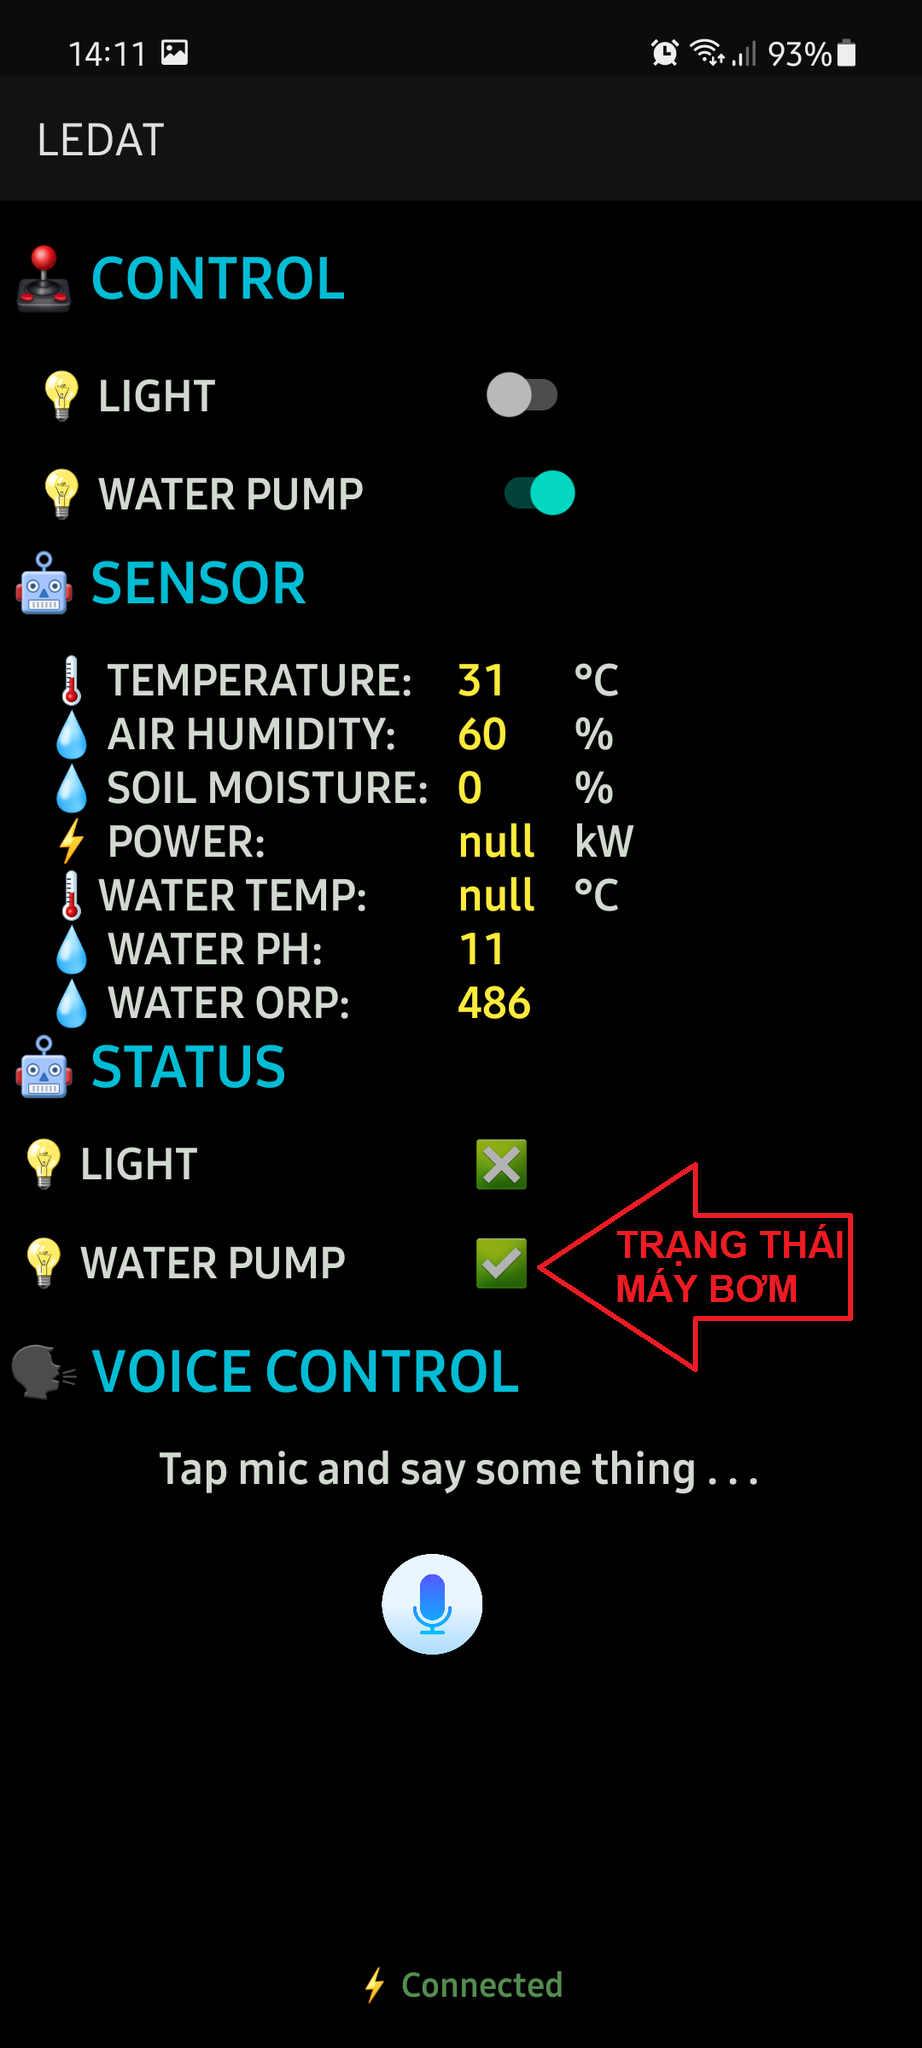
\includegraphics[scale=0.2]{Chapter 4/image chapter 4/appR1OFFR2ON.png}
	\caption[Trang thái của end-Node được hiển thị trên app]{Trang thái của end-Node được hiển thị trên app}
	\label{hinh49}
\end{figure}
\begin{figure}[H]
	\centering
	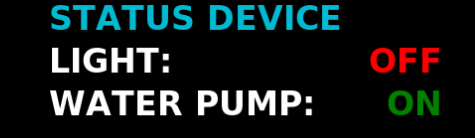
\includegraphics[scale=0.3]{Chapter 4/image chapter 4/Relay1OFF-Relay2ON.png}
	\caption[Trang thái của end-Node được hiển thị trên Gateway]{Trang thái của end-Node được hiển thị trên Gateway}
	\label{hinh410}
\end{figure}